\documentclass[conference]{IEEEtran}
\usepackage{times}

% numbers option provides compact numerical references in the text. 
\usepackage[numbers]{natbib}
\usepackage{multicol}
\usepackage[bookmarks=true]{hyperref}

\pdfinfo{
   /Author (Homer Simpson)
   /Title  (Robots: Our new overlords)
   /CreationDate (D:20101201120000)
   /Subject (Robots)
   /Keywords (Robots;Overlords)
}

\begin{document}

% paper title
\title{Template paper for the \\Robotics: Science and Systems Conference}

% You will get a Paper-ID when submitting a pdf file to the conference system
\author{Author Names Omitted for Anonymous Review. Paper-ID [add your ID here]}

%\author{\authorblockN{Michael Shell}
%\authorblockA{School of Electrical and\\Computer Engineering\\
%Georgia Institute of Technology\\
%Atlanta, Georgia 30332--0250\\
%Email: mshell@ece.gatech.edu}
%\and
%\authorblockN{Homer Simpson}
%\authorblockA{Twentieth Century Fox\\
%Springfield, USA\\
%Email: homer@thesimpsons.com}
%\and
%\authorblockN{James Kirk\\ and Montgomery Scott}
%\authorblockA{Starfleet Academy\\
%San Francisco, California 96678-2391\\
%Telephone: (800) 555--1212\\
%Fax: (888) 555--1212}}


% avoiding spaces at the end of the author lines is not a problem with
% conference papers because we don't use \thanks or \IEEEmembership


% for over three affiliations, or if they all won't fit within the width
% of the page, use this alternative format:
% 
%\author{\authorblockN{Michael Shell\authorrefmark{1},
%Homer Simpson\authorrefmark{2},
%James Kirk\authorrefmark{3}, 
%Montgomery Scott\authorrefmark{3} and
%Eldon Tyrell\authorrefmark{4}}
%\authorblockA{\authorrefmark{1}School of Electrical and Computer Engineering\\
%Georgia Institute of Technology,
%Atlanta, Georgia 30332--0250\\ Email: mshell@ece.gatech.edu}
%\authorblockA{\authorrefmark{2}Twentieth Century Fox, Springfield, USA\\
%Email: homer@thesimpsons.com}
%\authorblockA{\authorrefmark{3}Starfleet Academy, San Francisco, California 96678-2391\\
%Telephone: (800) 555--1212, Fax: (888) 555--1212}
%\authorblockA{\authorrefmark{4}Tyrell Inc., 123 Replicant Street, Los Angeles, California 90210--4321}}


\maketitle

\begin{abstract}
We consider the problem of learning to manipulate deformable objects
through learning from demonstrations.  Recent
work~\cite{Schulmanetal_IROS2013, Schulmanetal_ISRR2013} has shown
promising results in enabling robotic manipulation of deformable
objects through learning from demonstrations.  Their approach is able
to generalize from a single demonstration, and suggests a nearest
neighbor approach to decide which demonstration to generalize from for
a given test situation.  Such a nearest neighbor approach, however,
ignores important aspects of the problem:  brittleness (versus
robustness) of demonstrations when generalized through this process,
and the extent to which a demonstration makes progress towards the goal.

In this paper, we present a max-margin q-learning-based solution
to the demonstration selection problem that
can account for the variability in robustness of demonstrations and the
sequential nature of our tasks.   We also present experimental
validation of our approach.  We developed a knot-tying benchmark for
evaluating the effectiveness of
our proposed approach.   The
nearest neighbor approach described in \citet{Schulmanetal_ISRR2013} achieves a
68.8\% success rate. Our approach achieves a success rate of 95.2\%.
\end{abstract}


\IEEEpeerreviewmaketitle

\section{Introduction}
The recent commercial availablity of relatively cheap mobile robots such as Baxter and the UBR 1 
creates a very real possiblity for widespread appliation of robotics to mobile manipulation tasks.
There are huge economic gains to be had from the deployment of robotics in settings that range from homes to factories.
Our goal is to endow robots with the ability to execute complex, goal-directed, tasks in these unstructured settings.

These problems are characterized by state and action spaces that are high-dimensional and continuous.
The computational complexity faced by a robotic agent makes general solution of these problems difficult.
In modern factories, this is mitigated through intelligent design of environments and manipulation policies.
However, the design time and the skill required on the part of system designers prohibits application of these approaches for unstructured settings and more complex task.
Deformable object manipulation present an especially challenging scenario as modelling or tracking the underlying state of the world is a challenging task \cite{SchulmanLeeHoAbbeel_ICRA2013,Javdanietal_2011,Haehnel03a}.

One way to mitigate these issues is to frame our problem as one of learning from demonstrations.
Rather than starting from scratch in each scenario, we generalize from an expert demonstration.

A recent approach makes use of \emph{trajectory transfer} through the use of non-rigid registration to solve this problem.
When faced with a novel scenario, trajectory tranfers fits a function $f:\mathbb{R}^3 \rightarrow \mathbb{R}^3$ that warps a demonstration scene to a novel setting.
The demonstrated trajectory is then warped with this function and the result is executed. 
This has been shown to be effective for many complex task, including knot-tying and suturing \cite{Schulmanetal_ISRR2013, Schulmanetal_IROS2013}.\dhm{needs several citations}

There are limits to how well a single trajectory can transfer. 
Instead we provide a library of demonstrations and a method that selects which trajectory to transfer.
This enables our trajectory transfer systems to perform complex tasks by sequencing several trajecotry generalizations.
Selecting a demonstration that will generalize well to a particular scenario is integral to successful trajectory transfer and presents a tought challenge. 
Certain trajectories will generalize better than others and particular sequences of demonstrations may perform tasks more efficiently than others.
Current approaches make use of a nearest-neighbor policy that does not account for these features of the problem and fail to solve many problems that are solvable with that set of demonstrations.

\begin{figure}[t]
  \centering
    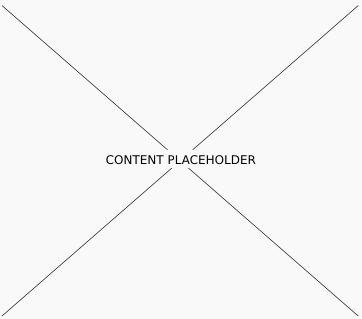
\includegraphics[width=0.9\linewidth]{figures/placeholder.png}
  \caption{Cute picture of robot tying knot}
  \label{fig:frontfig}
\end{figure}

In this paper, we present a solution to the demonstration selection problem that can account for the generalizability of demonstrations and the sequential nature of our applications.
Given a set of demonstrations and a method for generalizing them, we construct a discrete action abstract MDP.
Each action in this MDP is associated with a demonstration and our transition function is defined as applying trajectory transfer to generalize that demonstration.

This construction allows us to learn a Q function from example sequences of state-demonstration pairs.
This is accomplished through a max margin optimization problem whose solution captures the optimality of the examples and the temporal constraints imposed by the sequential nature of our tasks.
Our objective is a linear combination of features which are completely task agnostic and can be applied to any problem where trajectory transfer applies. 
We investigate the utility of this approach in a challenging knot-tieing scenario and show that the greedy application of our learned policy outperforms the nearest-neighbor baseline on a challenging distribution of problems. 
We leverage the fact that we learn a Q function representation of our policy (as opposed to a direct mapping from features to actions) to use a beam search to get near perfect performance in this task.
Finally, we present a method for bootstraping, though a process we call Leave-One-Out-Labelling, that enables us to do Max Margin Q-Learning with no additional human supervision beyond the initial demonstrations.

The rest of this paper is organized as follows: \dhm{fill this in later once we've drafted everything else}




\section{Related Work}
Related work for our contribution stems from three areas of research: deformable object manipulation (in particular knot-tieing), max margin policy learning, and \dhm{BLAH}
\subsection{Deformable Object Manipulation}
Our approach can be applied towards a variety of tasks in robotics,
including the manipulation of deformable objects.
In particular, we demonstrate the effectiveness of our approach for
knot tying, a commonly studied manipulation task in robotics.
Previous approaches to knot tying usually depend on rope-specific knowledge
and assumptions.
For instance, in knot planning from observation (KPO), knot theory is used
to recognize rope configurations and define movement primitives in visual
observations of humans tying knots \cite{Morita_ICRA2003, Takamatsu_TransRob2006}.
Existing motion planning approaches for knot tying use topological
representations of rope states (i.e. sequences of rope crossings and their
properties) and define a model for transitioning between topological states
\cite{Saha_ExpRobotics2008, Wakamatsu_IJRR2006}.
Robust open loop execution of knot tying has also been explored \cite{Bell_PhD2010}.

Recently, Schulman et al. used trajectory transfer to enable learning
from human-guided demonstrations of knot tying \cite{Schulmanetal_ISRR2013}.
For a given rope configuration, trajectory transfer is applied to the nearest
demonstration, and the resulting trajectory is executed.
The distance metric used is the thin plate spline (TPS) registration
cost between the rope configurations in the new scene and demonstration.
However, certain demonstrations may be less robust than others: for example,
a demonstration trajectory may involve a grasp that is unnecessarily near
the edge of a rope.
Our approach uses WillSmith to learn a policy that more robustly selects a
demonstration to apply, instead of always selecting the nearest demonstration.
\subsection{Max Margin Policy Learning}

\subsection{Inverse Optimal Control}
\et{I'm not really sure this is a subsection we want, just putting this here for
  now so the next sentence has a home.}  \citet{Dvijotham_ICML2010} also attempt
to directly learn a value function or Q-function for a MDP given sample
transitions generated by an optimal control policy. However, they assume either
a discrete state space or a linear dynamics model. In contrast, our method makes
no assumptions about the size of the state space or the dynamics model, instead
relying on segments of expert demonstrations as a means of navigating the state
space efficiently. \et{Someone who actually understands robotics should probably
  check this statement.}


\section{Section}

Section text here. 

\subsection{Subsection Heading Here}
Subsection text here.

\subsubsection{Subsubsection Heading Here}
Subsubsection text here.


\section{RSS citations}

Please make sure to include \verb!natbib.sty! and to use the
\verb!plainnat.bst! bibliography style. \verb!natbib! provides additional
citation commands, most usefully \verb!\citet!. For example, rather than the
awkward construction 

{\small
\begin{verbatim}
\cite{kalman1960new} demonstrated...
\end{verbatim}
}

\noindent
rendered as ``\cite{kalman1960new} demonstrated...,''
or the
inconvenient 

{\small
\begin{verbatim}
Kalman \cite{kalman1960new} 
demonstrated...
\end{verbatim}
}

\noindent
rendered as 
``Kalman \cite{kalman1960new} demonstrated...'', 
one can
write 

{\small
\begin{verbatim}
\citet{kalman1960new} demonstrated... 
\end{verbatim}
}
\noindent
which renders as ``\citet{kalman1960new} demonstrated...'' and is 
both easy to write and much easier to read.
  
\subsection{RSS Hyperlinks}

This year, we would like to use the ability of PDF viewers to interpret
hyperlinks, specifically to allow each reference in the bibliography to be a
link to an online version of the reference. 
As an example, if you were to cite ``Passive Dynamic Walking''
\cite{McGeer01041990}, the entry in the bibtex would read:

{\small
\begin{verbatim}
@article{McGeer01041990,
  author = {McGeer, Tad}, 
  title = {\href{http://ijr.sagepub.com/content/9/2/62.abstract}{Passive Dynamic Walking}}, 
  volume = {9}, 
  number = {2}, 
  pages = {62-82}, 
  year = {1990}, 
  doi = {10.1177/027836499000900206}, 
  URL = {http://ijr.sagepub.com/content/9/2/62.abstract}, 
  eprint = {http://ijr.sagepub.com/content/9/2/62.full.pdf+html}, 
  journal = {The International Journal of Robotics Research}
}
\end{verbatim}
}
\noindent
and the entry in the compiled PDF would look like:

\def\tmplabel#1{[#1]}

\begin{enumerate}
\item[\tmplabel{1}] Tad McGeer. \href{http://ijr.sagepub.com/content/9/2/62.abstract}{Passive Dynamic
Walking}. {\em The International Journal of Robotics Research}, 9(2):62--82,
1990.
\end{enumerate}
%
where the title of the article is a link that takes you to the article on IJRR's website. 


Linking cited articles will not always be possible, especially for
older articles. There are also often several versions of papers
online: authors are free to decide what to use as the link destination
yet we strongly encourage to link to archival or publisher sites
(such as IEEE Xplore or Sage Journals).  We encourage all authors to use this feature to
the extent possible.

\section{Conclusion} 
\label{sec:conclusion}

The conclusion goes here.

\section*{Acknowledgments}

%% Use plainnat to work nicely with natbib. 

\bibliographystyle{plainnat}
\bibliography{references}

\end{document}


